g\documentclass{article}
\usepackage{graphicx}
\usepackage[margin=0.5in]{geometry}
\usepackage{mathtools}

\begin{document}

\title{Ph20 Lab 2: Intro to Numerical Techniques}
\author{Neil McBlane: 2050386}

\maketitle

\section*{Question 1: Extended Simpson's formula}
Simpson's formula for integrating $f(x)$ between points $x=a$ and $x=b$ is given by:
\begin{equation}
\label{equ:simp}
  \int_a^b f(x)dx = H\left(\frac{f(a)}{6} + \frac{4f(c)}{6} + \frac{f(b)}{6}\right)
\end{equation}
Where $c = \frac{b-a}{2}$. To evaluate the error, we must consider an approximation up to 4th order in $f(x)$, so we Taylor expand our terms:
\begin{equation}
  f(b) = f(a) + f'(a)H + \frac{f''(a)}{2!}H^2 + \frac{f'''(a)}{3!}H^3 + \frac{f''''(\eta)}{4!}H^4
\end{equation} 
\begin{equation}
  f(c) = f(a) + f'(a)\frac{H}{2} + \frac{f''(a)}{2!}\left(\frac{H}{2}\right)^2 + \frac{f'''(a)}{3!}\left(\frac{H}{2}\right)^3 + \frac{f''''(\eta)}{4!}\left(\frac{H}{2}\right)^4
\end{equation}
Where $\eta$ is the Lagrangian remainder. Combining these with Equation \ref{equ:simp} we have an estimated integral of:
\begin{equation}
\label{equ:simpapprox}
  I_{simp} = H\left(f(a) + \frac{f'(a)}{2}H + \frac{f''(a)}{6}H^2 + \frac{f'''(a)}{24}H^3 + \frac{5f''''(\eta)}{576}H^4\right)
\end{equation}
Taylor expanding the exact integral to the same order gives:
\begin{equation}
  I = H\left(f(a) + \frac{f'(a)}{2}H + \frac{f''(a)}{6}H^2 + \frac{f'''(a)}{24}H^3 + \frac{f''''(\eta)}{120}H^4\right)
\end{equation}
The difference between the approximation and exact value gives the error:
\begin{equation}
\label{equ:localerr}
 error_{loc} = I_{simp} - I = \frac{f''''(\eta)}{2880}H^5
\end{equation}
Which, as expected, is of order 5 in H.

The extended Simpson formula splits the region [a,b] into N equal sized chunks of size $h_N = \frac{b-a}{N}$. Splitting the integration into these parts too gives:
\begin{equation}
  \int_a^b f(x)dx = \int_{x_0}^{x_2} f(x)dx + \int_{x_2}^{x_4} f(x)dx + ... \int_{x_{2N-2}}^{x_{2N}} f(x)dx
\end{equation}
Applying Simpson's formula to each of these chunks:
\begin{equation}
  I_{simp} = h_N\left(\frac{f(x_0)}{6} + \frac{4f(x_1)}{6} + \frac{f(x_2)}{6}\right) + h_N\left(\frac{f(x_2)}{6} + \frac{4f(x_3)}{6} + \frac{f(x_4)}{6}\right) +... h_N\left(\frac{f(x_{2N-2})}{6} + \frac{4f(x_{2N-1})}{6} + \frac{f(x_{2N})}{6}\right) 
\end{equation}
We can rewrite this as:
\begin{equation}
 I_{simp} = h_N\left(\frac{f(x_0)}{6} + \frac{f(x_{2N})}{6} + \frac{2}{3}\displaystyle\sum_{i=0}^{N-1} f(x_{2i+1}) + \frac{1}{3}\displaystyle\sum_{i=1}^{N-1} f(x_{2j})\right)
\end{equation}

As we now have N equal sized chunks, the global error will just be N times the error given by Equation \ref{equ:localerr}, where instead the width is $h_N$:
\begin{equation}
 error_{glob} = \frac{f''''(\eta)}{2880}h_N^5 N = \frac{f''''(\eta)}{2880}h_N^5 \frac{H}{h_N} = H\frac{f''''(\eta)}{2880}h_N^4
\end{equation}

Which is of fourth order in $h_N$.

\clearpage

\section*{Question 4: Comparing Simpson's and the trapezoidal methods}

Figure \ref{fig:convergence} demonstrates that as the number of steps taken to complete the integration increases, both converge to the true value for $\int_0^1 e^x dx = 1.7182818284590452354$. We see a much faster convergence for Simpson's method, but both clearly approach the correct value. When N is large - for example 10,000 - the Trapezoidal method gives an error of $1\times10^{-8}\%$ and the Simpson method an error too small for iPython to handle.

\begin{figure}[h]
\centering
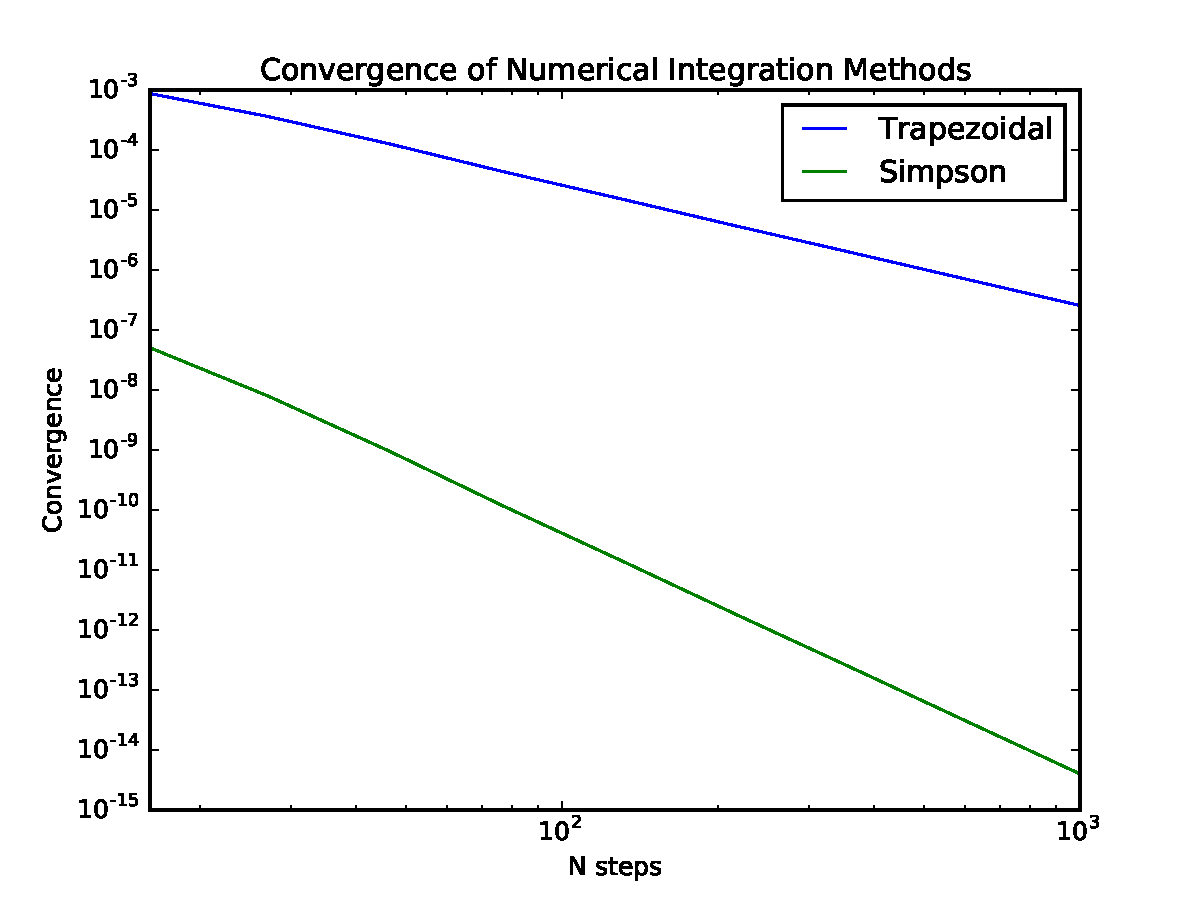
\includegraphics[width=0.6\textwidth]{images/err_convergence.pdf}
\caption{Convergence of the extended Simpson and extended Trapezoidal numerical integration methods to the true value of the integral of $e^x$ from 0 to 1 as the number of steps taken increases.}
\label{fig:convergence}
\end{figure}

\section*{Question 5: Relative accuracy}

The table below shows the number of steps required for the convergence to meet the specified accuracy. Comparison with Figure \ref{fig:convergence} shows that the function is performing as expected. Convergence occurs at around the same rate for $\cos(x)$

\begin{center}
\begin{tabular}{ |c||c|c| } 
 \hline
 Convergence & $e^x$ & $\cos(x)$ \\ 
 \hline
 $10^{-8}$   & $32$   & $32$  \\ 
 $10^{-10}$  & $128$  & $128$ \\
 $10^{-12}$  & $512$  & $512$ \\
 $10^{-14}$  & $1024$ & $1024$\\ 
 \hline
\end{tabular}
\end{center}

\section*{Question 6: Comparison to scipy}

Using scipy.integrate.quad(np.exp, 0, 1) returns an error of the order $1\times10^{-12}$, a massive improvement on the error obtained using our home-made Trapezoidal method - even at 10,000 steps. It is also signicicantly faster. Using the Romberg method gives an error of the same order, and is also significantly faster.

\end{document}
